\begin{figure}
  \centering
  \begin{subfigure}[b]{.45\linewidth}
    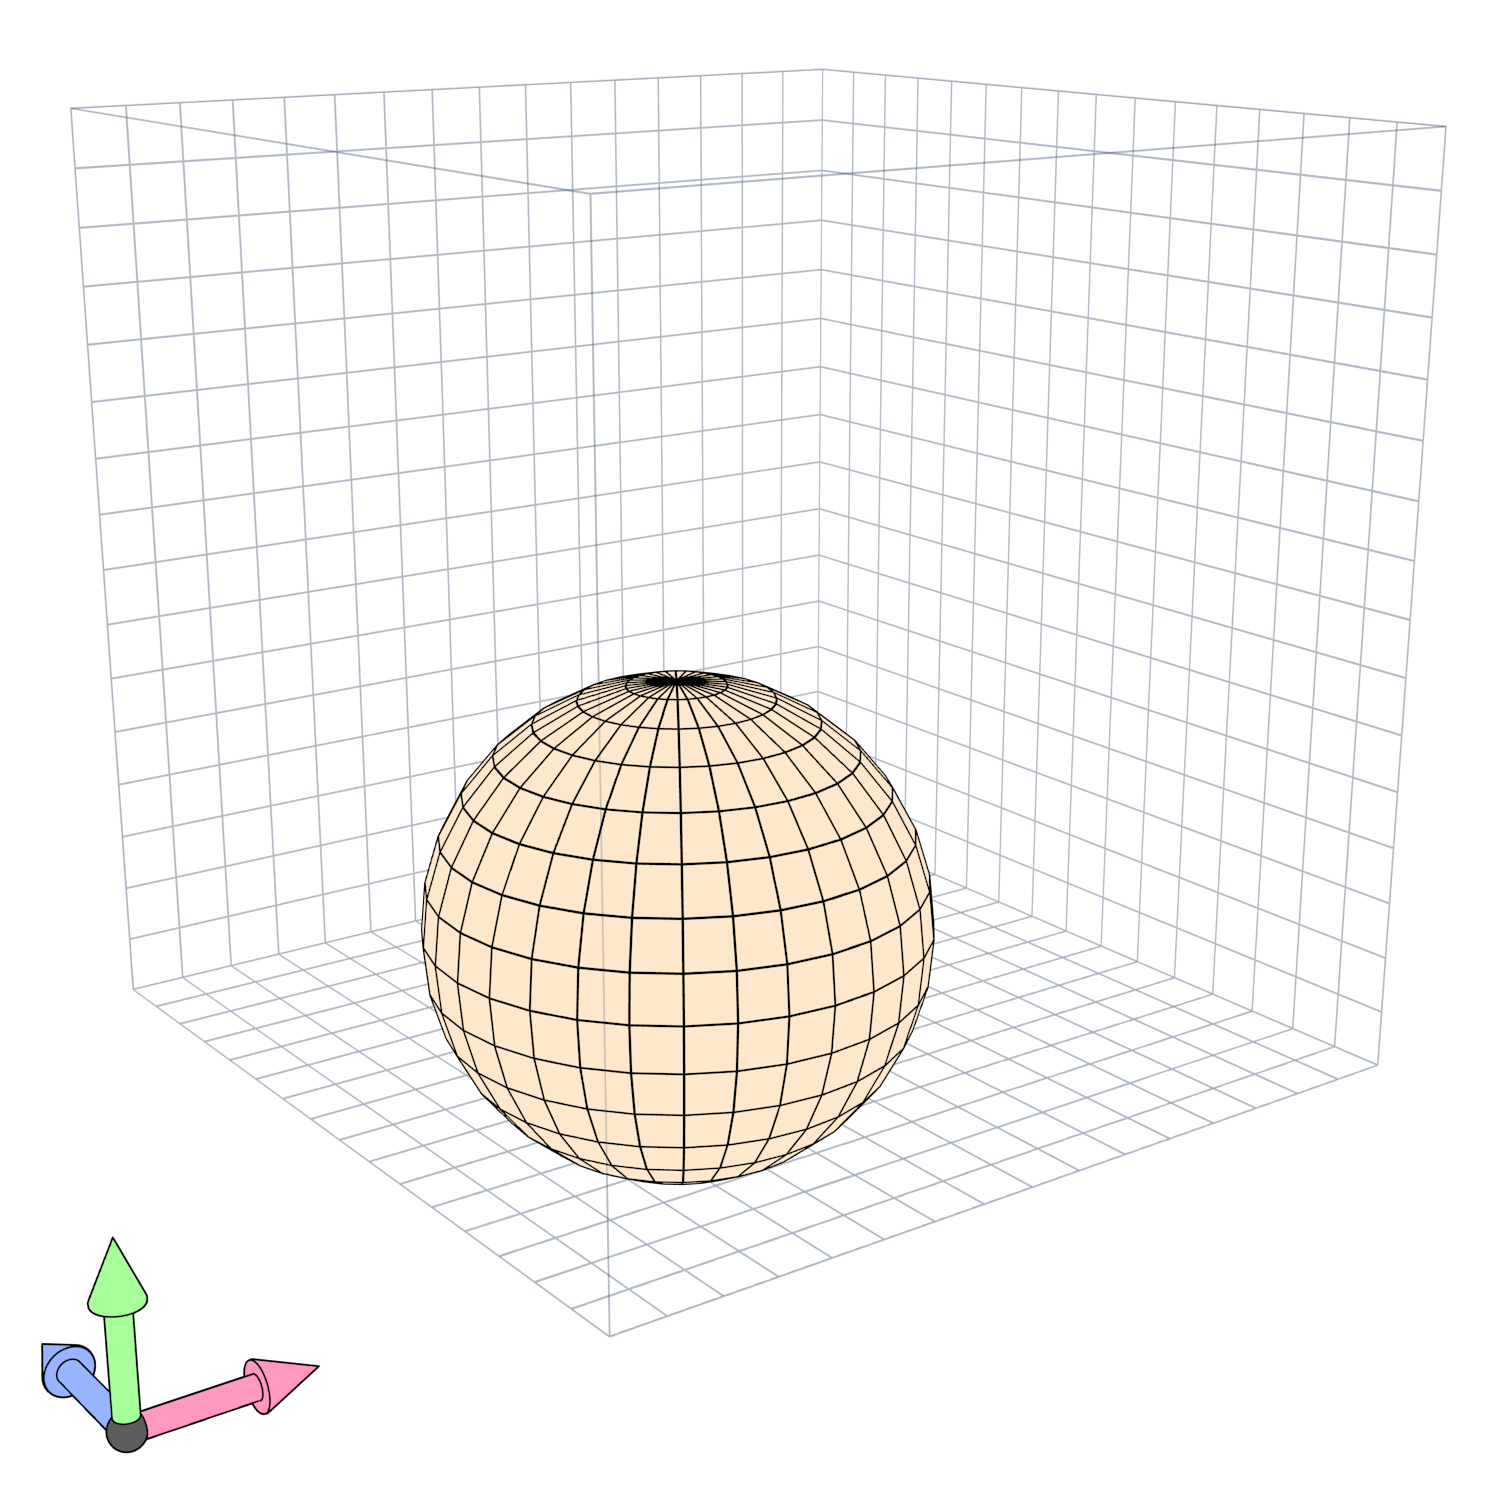
\includegraphics[width=\textwidth]{./img/raw/hs-slt_left.png}%
    \caption{licht volume}%
    \label{fig:hs-slt-left}%
  \end{subfigure}
  \begin{subfigure}[b]{.45\linewidth}%
    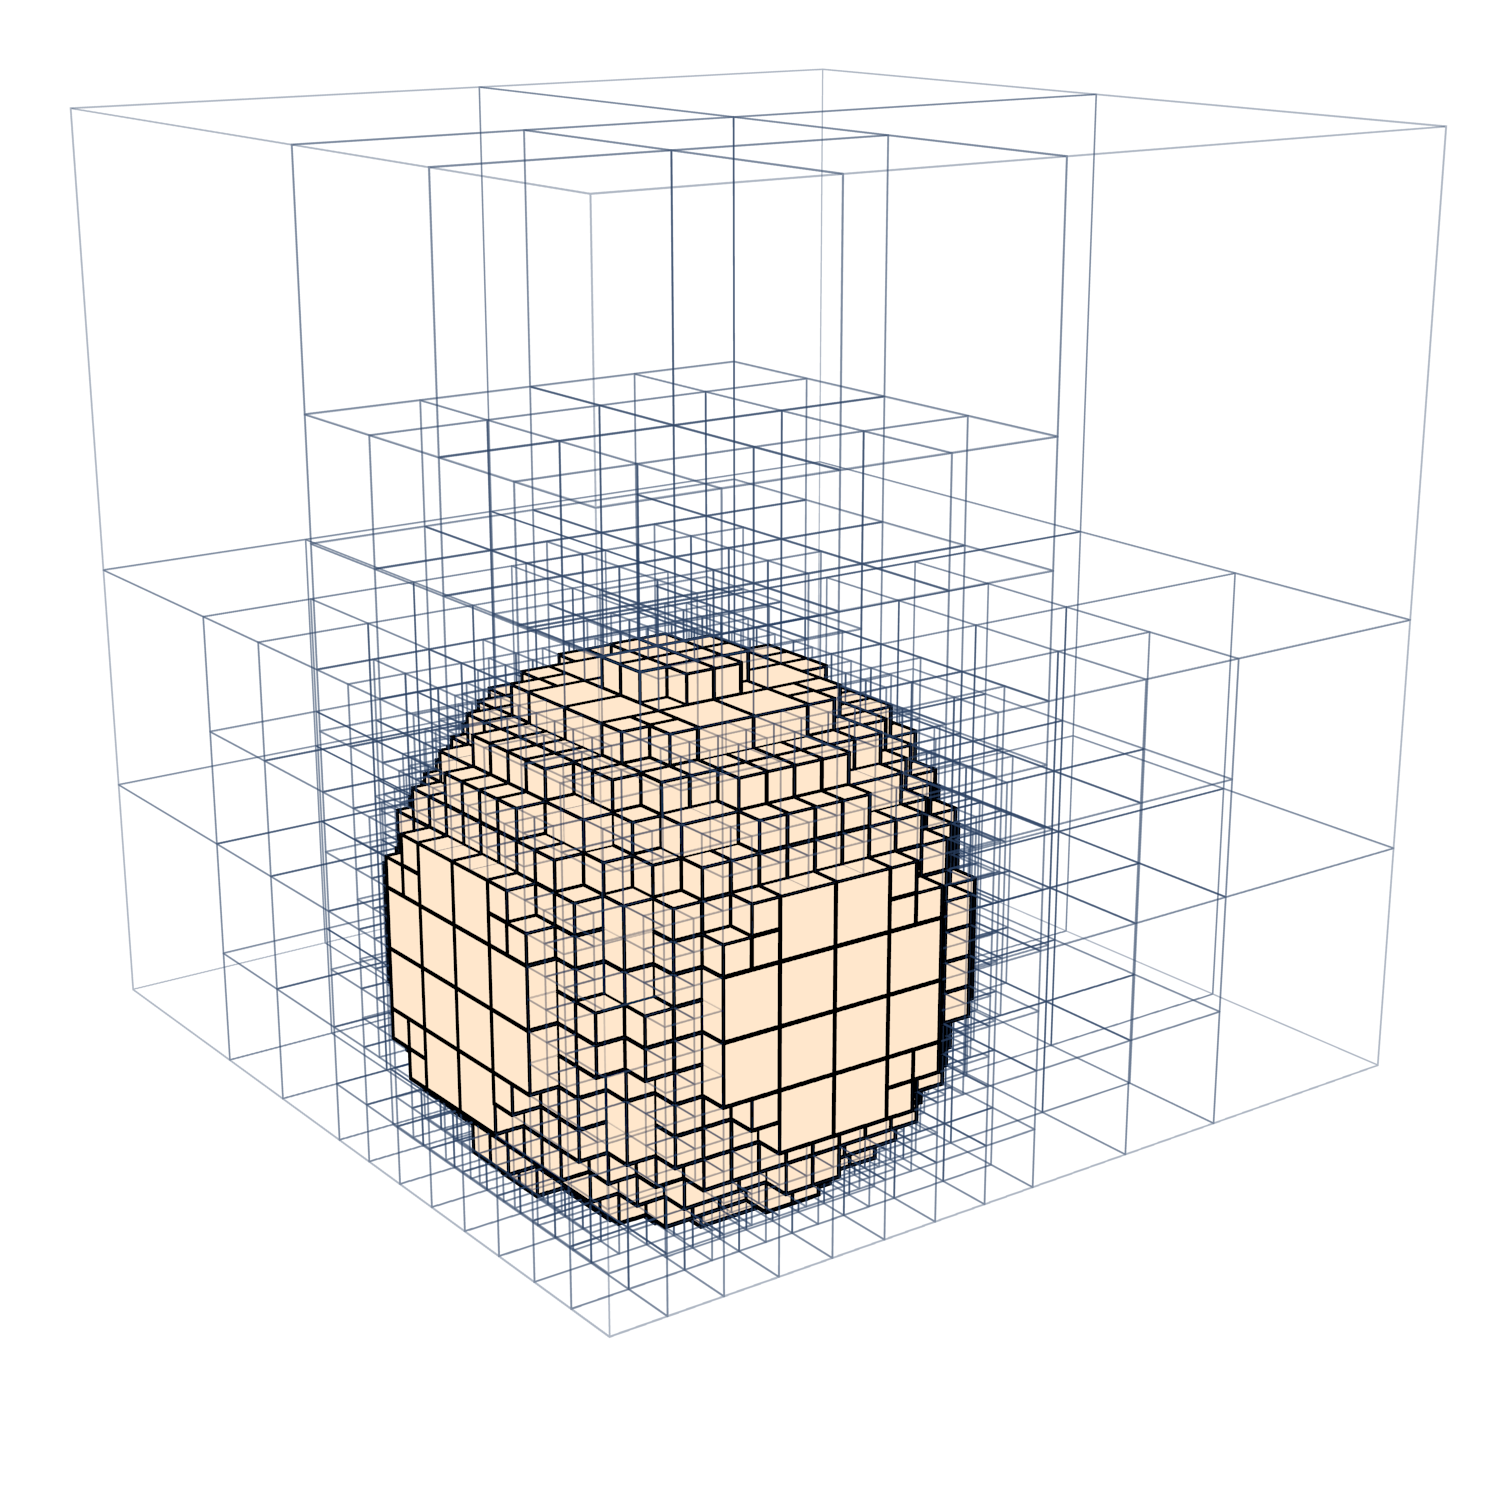
\includegraphics[width=\textwidth]{./img/raw/hs-slt_right.png}%
    \caption{enkele licht boom}%
    \label{fig:hs-slt-right}%
  \end{subfigure}
  \caption{Voorstelling van de enkele licht boom.}
  \label{fig:hs-slt}
\end{figure}
